\documentclass[border=6pt]{standalone}
\usepackage{tikz}
\usepackage[edges]{forest}
\usetikzlibrary{arrows.meta,positioning,calc,decorations.pathreplacing,shapes.geometric}
\begin{document}
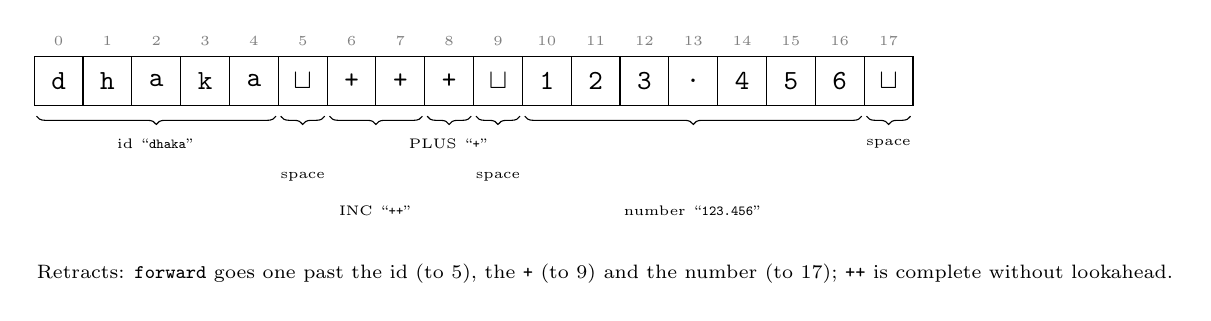
\begin{tikzpicture}[font=\small,cell/.style={draw,minimum size=0.62cm,inner sep=0pt,font=\ttfamily}]
\node[cell] at (0.00,0) {d};
\node[font=\tiny,gray] at (0.00,0.5) {0};
\node[cell] at (0.62,0) {h};
\node[font=\tiny,gray] at (0.62,0.5) {1};
\node[cell] at (1.24,0) {a};
\node[font=\tiny,gray] at (1.24,0.5) {2};
\node[cell] at (1.86,0) {k};
\node[font=\tiny,gray] at (1.86,0.5) {3};
\node[cell] at (2.48,0) {a};
\node[font=\tiny,gray] at (2.48,0.5) {4};
\node[cell] at (3.10,0) {$\sqcup$};
\node[font=\tiny,gray] at (3.10,0.5) {5};
\node[cell] at (3.72,0) {+};
\node[font=\tiny,gray] at (3.72,0.5) {6};
\node[cell] at (4.34,0) {+};
\node[font=\tiny,gray] at (4.34,0.5) {7};
\node[cell] at (4.96,0) {+};
\node[font=\tiny,gray] at (4.96,0.5) {8};
\node[cell] at (5.58,0) {$\sqcup$};
\node[font=\tiny,gray] at (5.58,0.5) {9};
\node[cell] at (6.20,0) {1};
\node[font=\tiny,gray] at (6.20,0.5) {10};
\node[cell] at (6.82,0) {2};
\node[font=\tiny,gray] at (6.82,0.5) {11};
\node[cell] at (7.44,0) {3};
\node[font=\tiny,gray] at (7.44,0.5) {12};
\node[cell] at (8.06,0) {.};
\node[font=\tiny,gray] at (8.06,0.5) {13};
\node[cell] at (8.68,0) {4};
\node[font=\tiny,gray] at (8.68,0.5) {14};
\node[cell] at (9.30,0) {5};
\node[font=\tiny,gray] at (9.30,0.5) {15};
\node[cell] at (9.92,0) {6};
\node[font=\tiny,gray] at (9.92,0.5) {16};
\node[cell] at (10.54,0) {$\sqcup$};
\node[font=\tiny,gray] at (10.54,0.5) {17};
\draw[decorate,decoration={brace,amplitude=3pt,mirror}] (-0.28,-0.45) -- (2.76,-0.45);
\node[font=\tiny,align=center,anchor=north,fill=white] at (1.24,-0.62) {id ``\texttt{dhaka}''};
\draw[decorate,decoration={brace,amplitude=3pt,mirror}] (2.82,-0.45) -- (3.38,-0.45);
\node[font=\tiny,align=center,anchor=north,fill=white] at (3.10,-1.04) {space};
\draw[decorate,decoration={brace,amplitude=3pt,mirror}] (3.44,-0.45) -- (4.62,-0.45);
\node[font=\tiny,align=center,anchor=north,fill=white] at (4.03,-1.46) {INC ``\texttt{++}''};
\draw[decorate,decoration={brace,amplitude=3pt,mirror}] (4.68,-0.45) -- (5.24,-0.45);
\node[font=\tiny,align=center,anchor=north,fill=white] at (4.96,-0.62) {PLUS ``\texttt{+}''};
\draw[decorate,decoration={brace,amplitude=3pt,mirror}] (5.30,-0.45) -- (5.86,-0.45);
\node[font=\tiny,align=center,anchor=north,fill=white] at (5.58,-1.04) {space};
\draw[decorate,decoration={brace,amplitude=3pt,mirror}] (5.92,-0.45) -- (10.20,-0.45);
\node[font=\tiny,align=center,anchor=north,fill=white] at (8.06,-1.46) {number ``\texttt{123.456}''};
\draw[decorate,decoration={brace,amplitude=3pt,mirror}] (10.26,-0.45) -- (10.82,-0.45);
\node[font=\tiny,align=center,anchor=north,fill=white] at (10.54,-0.62) {space};
\node[font=\scriptsize,anchor=west] at (-0.4,-2.45) {Retracts: \texttt{forward} goes one past the id (to 5), the \texttt{+} (to 9) and the number (to 17); \texttt{++} is complete without lookahead.};
\end{tikzpicture}
\end{document}
